%!TEX root = ../lectures.tex

\topic{Volumes by Slicing and Solids of Revolution}

The goal of this discussion is to explore how definite integrals can be used to express the volumes of certain three-dimensional solids.

\begin{figure}
	\centering
	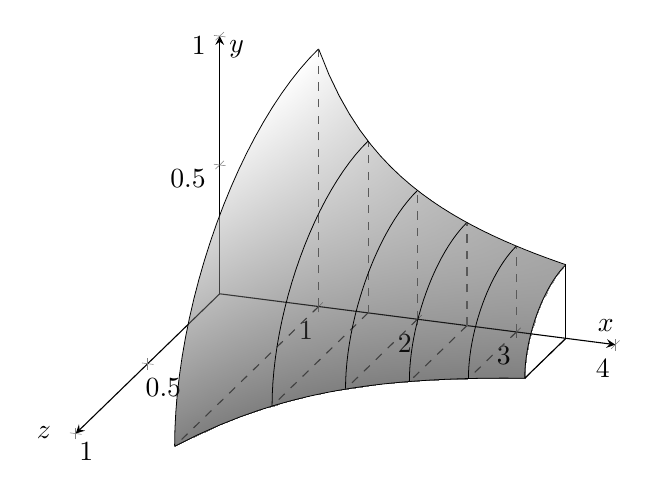
\begin{tikzpicture}
		\begin{axis}[
			view = {20}{30},
			axis lines = center,
			xlabel = $x$,
			ylabel = $z$,
			y dir = reverse,
			zlabel = $y$,
			xmin = 0,
			xmax = 4,
			ymin = 0,
			ymax = 1,
  		every axis y label/.append style = {at = (ticklabel* cs:0)}]
			zmin = 0,
			zmax = 1.3,
			]
			\addplot3[
			surf,
			colormap = {blackwhite}{gray(0cm) = (0); gray(1cm) = (1)},
			shader = interp,
			samples = 50,
			domain = 1:3.5,
			y domain = 0:pi/2,
			z buffer = sort,
			opacity = 0.5
			](x, {(1/x) * cos(deg(y))}, {(1/x) * sin(deg(y))});

			\foreach \xx in {1.0, 1.5, ..., 3.5}
      {
        \addplot3+[
				domain = 0:pi/2,
				%y domain = 0:pi/2,
				line width = 0.1mm,
				mark = none,
				color = black,
				samples y = 0,
				solid
				]({\xx}, {(1/\xx) * cos(deg(x))}, {(1/\xx) * sin(deg(x))});
				\addplot3[
				black!75,
				dashed
				] coordinates {(\xx, 0, 0) (\xx, 1/\xx, 0)};
				\addplot3[
				black!65,
				dashed
				] coordinates {(\xx, 0, 0) (\xx, 0, 1/\xx)};
      }
			\addplot3[
			black,
			solid
			] coordinates {(3.5, 0, 0) (3.5, 1/3.5, 0)};
			\addplot3[
			black,
			solid
			] coordinates {(3.5, 0, 0) (3.5, 0, 1/3.5)};
			\foreach \yy in {0, pi/2}
      {
         \addplot3[
				 domain = 1:3.5,
				 line width = 0.1mm,
				 mark = none,
				 color = black,
				 samples y = 0
				 ]({x}, {(1/x) * cos(deg(\yy))}, {(1/x) * sin(deg(\yy))});
      }
		\end{axis}
	\end{tikzpicture}
	\caption{A volume with the $x$ interval $\interval{1}{3.5}$ partitioned into equal parts.}
	\label{lec13:exvolume}
\end{figure}

The basic idea is simple and similar to how we defined areas under curves.
Consider Figure \ref{lec13:exvolume}, and let $A(x)$ (continuous, let's say) describe the area of the cross-sectional area of the solid at a given $x$ value.

Then by partitioning $\interval{a}{b}$ into $n$ parts,
\[
	a = x_0 < x_1 < x_2 < \ldots < x_n = b
\]
we have an approximate volume
\[
	V = \sum_{i = 1}^n A(x_i) \Delta x_i.
\]

\noindent
By refining the partition, just as we're used to for areas, we get
\[
	V = \int_a^b A(x) \, d x.
\]

\noindent
We are interested in a special case of this, where the cross-sections are circular.
We call such objects \keyword{solids of revolution}\index{solid of revolution}, because one can generate them by rotating a region of the plane around an axis of that plane.

\begin{figure}[b]
	\centering
	\begin{subfigure}{0.4\linewidth}
		\centering
		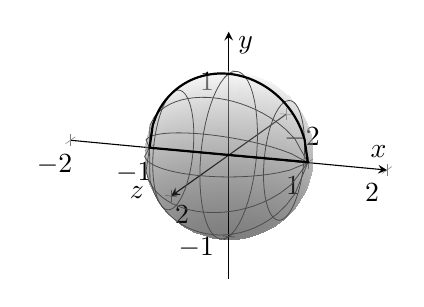
\begin{tikzpicture}
			\begin{axis}[
				scale = 0.8,
				view = {20}{15},
				axis lines = center,
				axis equal,
				xlabel = $x$,
				ylabel = $z$,
				y dir = reverse,
				zlabel = $y$,
				xmin = -1,
				xmax = 1,
				ymin = -2,
				ymax = 2,
	  		every axis y label/.append style = {at = (ticklabel* cs:0)}]
				zmin = -1,
				zmax = 1,
				]
				\addplot3[
				surf,
				colormap = {blackwhite}{gray(0cm) = (0); gray(1cm) = (1)},
				shader = interp,
				samples = 50,
				domain = -1:1,
				y domain = 0:2*pi,
				z buffer = sort,
				opacity = 0.5
				](x, {sqrt(1-x^2) * cos(deg(y))}, {sqrt(1-x^2) * sin(deg(y))});
				\foreach \xx in {-0.7, 0, 0.7}
	      {
	        \addplot3+[
					domain = 0:2*pi,
					line width = 0.1mm,
					mark = none,
					black!70,
					samples y = 0,
					samples = 50
					](\xx, {sqrt(1-(\xx)^2) * cos(deg(x))}, {sqrt(1-(\xx)^2) * sin(deg(x))});
	      }
				\foreach \yy in {-1.0, -0.5, ..., 1}
	      {
	        \addplot3[
					domain = -1:1,
					line width = 0.1mm,
					mark = none,
					black!70,
					samples y = 10
					](x, {sqrt(1-(x)^2) * cos(deg(\yy))}, {sqrt(1-(x)^2) * sin(deg(\yy))});
	      }

				\addplot3[
				samples = 50,
				domain = -1:1,
				y domain = 0:2*pi,
				black,
				solid,
				thick
				](x, 0, {sqrt(1-x^2)});
			\end{axis}
		\end{tikzpicture}
		\caption{Sphere}
		\label{lec13:sphere}
	\end{subfigure}\qquad
	\begin{subfigure}{0.4\linewidth}
		\centering
		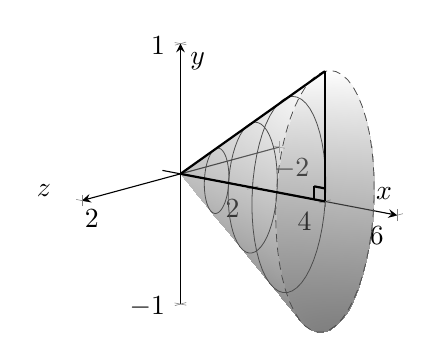
\begin{tikzpicture}
			\begin{axis}[
				scale = 0.8,
				view = {40}{15},
				axis lines = center,
				xlabel = $x$,
				ylabel = $z$,
				y dir = reverse,
				zlabel = $y$,
				xmin = -0.5,
				xmax = 6,
				ymin = -2,
				ymax = 2,
	  		every axis y label/.append style = {at = (ticklabel* cs:0)}]
				zmin = -1,
				zmax = 1,
				]
				\addplot3[
				surf,
				colormap = {blackwhite}{gray(0cm) = (0); gray(1cm) = (1)},
				shader = interp,
				samples = 50,
				domain = 0:4,
				y domain = 0:2*pi,
				z buffer = sort,
				opacity = 0.5
				](x, {x/4 * cos(deg(y))}, {x/4 * sin(deg(y))});
				\foreach \xx in {0, 1, ..., 4}
	      {
	        \addplot3+[
					domain = 0:2*pi,
					line width = 0.1mm,
					mark = none,
					black!70,
					samples y = 0,
					samples = 50
					](\xx, {\xx/4 * cos(deg(x))}, {\xx/4 * sin(deg(x))});
	      }

				\addplot3[
				samples = 50,
				domain = 0:4,
				y domain = 0:2*pi,
				black,
				solid,
				thick
				](x, 0, {x/4});
				\addplot3[
				black,
				solid,
				thick
				]coordinates{(0, 0, 0) (4, 0, 0)};
				\addplot3[
				black,
				solid,
				thick
				]coordinates{(4, 0, 0) (4, 0, 1)};
				\addplot3[
				black,
				solid,
				thick
				]coordinates{(3.7, 0, 0) (3.7, 0, 0.1)};
				\addplot3[
				black,
				solid,
				thick
				]coordinates{(3.7, 0, 0.1) (4, 0, 0.1)};
			\end{axis}
		\end{tikzpicture}
		\caption{Circular cone}
		\label{lec13:circularcone}
	\end{subfigure}
	\caption{Two solids of revolution.}
	\label{lec13:exsolidsofrevolution}
\end{figure}

For instance, by rotating a half disc about its diameter, one generates a solid sphere (see Figure \ref{lec13:sphere}, with the half disc outlined) and by rotating a right-angled triangle about one of its legs we get a circular cone (see Figure \ref{lec13:circularcone}, again with the base object outlined).

Now let us compute the volume of such objects.
If we let a region be bounded by $y = f(x)$, $y = 0$, $x = a$, and $x = b$, and then rotated about the $x$-axis, then the cross-section at $x$ is a circular disc with radius $\abs{f(x)}$.
The cross-sectional area is therefore
\[
	A(x) = \pi \abs{f(x)}^2 = \pi (f(x))^2,
\]
making the volume of this solid of revolution
\[
	V(x) = \pi \int_a^b (f(x))^2 \, d x.
\]

\begin{example}
	Find the volume of the solid sphere with radius $r$.

	We consider Figure \ref{lec13:sphere}, meaning that we generate the solid using the half-disc $0 \leq y \leq \sqrt{r^2 - x^2}$ for $-r \leq x \leq r$, rotating around the $x$-axis.

	We therefore get the volume
	\begin{align*}
		V &= \pi \int_{-r}^r \sqrt{r^2 - x^2}^2 \, d x = \pi \int_{-r}^r r^2 - x^2 \, dx  = 2 \pi \int_0^r r^2 - x^2 \, d x \\
		  &= 2 \pi \Big ( r^2 x - \frac{x^3}{3} \Big ) \biggr \rvert_0^r = 2 \pi \Big ( r^3 - \frac{1}{3} r^3) = 2 \pi \frac{2r^3}{3} = \frac{4}{3} \pi r^3. \qedhere
	\end{align*}
\end{example}

\begin{example}
	Find the volume of the right-circular cone with base radius $r$ and height $h$.

	As visualised in Figure \ref{lec13:circularcone} we construct right triangle with base $h$ and height $r$, and describe the line of its hypotenuse by a straight line equation, namely $y = r/h \cdot x$.
	We then rotate the region enclosed by this line, the $y$-axis, and $x = h$ about the $x$-axis.

	This gives the volume
	\begin{align*}
		V &= \pi \int_0^h \Big ( \frac{r}{h} x \Big )^2 \, d x = \pi \frac{r^2}{h^2} \int_0^h x^2 \, d x = \pi \frac{r^2}{h^2} \Big ( \frac{x^3}{3} \Big ) \biggr \rvert_0^h \\
		  &= \frac{\pi r^2}{3 h^2} h^3 = \frac{1}{3} \pi r^2 h. \qedhere
	\end{align*}
\end{example}

\noindent
Very curious things can happen here.

\begin{figure}[b]
	\centering
	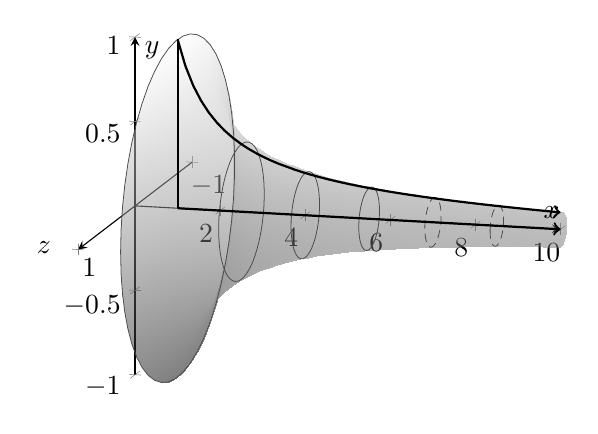
\begin{tikzpicture}
		\begin{axis}[
			view = {15}{15},
			axis lines = center,
			xlabel = $x$,
			ylabel = $z$,
			y dir = reverse,
			zlabel = $y$,
			xmin = 0,
			xmax = 10,
			ymin = -1,
			ymax = 1,
  		every axis y label/.append style = {at = (ticklabel* cs:0)}]
			zmin = -2,
			zmax = 2,
			]
			\addplot3[
			surf,
			colormap = {blackwhite}{gray(0cm) = (0); gray(1cm) = (1)},
			shader = interp,
			samples = 50,
			domain = 1:10,
			y domain = 0:2*pi,
			z buffer = sort,
			opacity = 0.5
			](x, {1/x * cos(deg(y))}, {1/x * sin(deg(y))});
			\foreach \xx in {1, 2.5, ..., 9}
      {
        \addplot3+[
				domain = 0:2*pi,
				line width = 0.1mm,
				mark = none,
				black!70,
				samples y = 0,
				samples = 50
				](\xx, {1/\xx * cos(deg(x))}, {1/\xx * sin(deg(x))});
      }
			\addplot3[
			samples = 50,
			domain = 1:10,
			y domain = 0:0,
			black,
			solid,
			thick,
			->
			](x, 0, 1/x);
			\addplot3[
			black,
			solid,
			thick,
			->
			]coordinates{(1, 0, 0) (10, 0, 0)};
			\addplot3[
			black,
			solid,
			thick
			]coordinates{(1, 0, 0) (1, 0, 1)};
		\end{axis}
	\end{tikzpicture}
	\caption{Gabriel's horn.}
	\label{lec13:gabrielshorn}
\end{figure}

\begin{example}[Gabriel's horn]
	Consider the infinitely long horn generated by rotating the region bounded by $y = 1/x$, $y = 0$, and to the right of $x = 1$, around the $x$-axis, as depicted in Figure \ref{lec13:gabrielshorn}.

	We show first that the surface area of this object is infinite.
	We haven't discussed explicitly how to do this, but intuitively it makes sense that we take the height of the object at a given $x$ value, multiply it by $2 \pi$ in order to get the circumference at this point, and multiply by some measurement of the length along the surface we travel if we step $d x$ to the right.\footnote{The full formula is $A = 2 \pi \int_a^b f(x) \sqrt{1 - (f'(x))^2} \, d x$, wherein one thinks of the length as the length of the hypotenuse of a triangle approximating what we're interested in.}

	Thus we have something along the lines of
	\[
		A = 2\pi \lim_{\alpha \to \infty} \int_1^\alpha \frac{1}{x} L(x) \, d x,
	\]
	with $L(x)$ being the length of the curve between $x$ and $x + d x$.
	The trick, now, is to observe that if we ignore this length term, we can't make the integrand greater, so
	\[
		A > 2\pi \lim_{\alpha \to \infty} \int_1^\alpha \frac{1}{x} \, d x = 2 \pi \lim_{\alpha \to \infty} \ln(\alpha) = \infty,
	\]
	yet
	\[
		V = \pi \lim_{\alpha \to \infty} \int_1^\alpha \frac{1}{x^2} \, d x = - \pi \lim_{\alpha \to \infty} \frac{1}{x} \biggr \rvert_1^\alpha = - \pi \lim_{\alpha \to \infty} \Big ( \frac{1}{\alpha} - 1 \Big ) = \pi.
	\]

	\noindent
	In some sense this means that we can fill the horn with a finite amount of paint, but it we tried to paint the inner surface of it we'd need an infinite amount.

	It is also interesting to note that the study of properties of this object, including this apparent paradox we present here, predate calculus.
\end{example}

\noindent
Sometimes we instead want to rotate around the $y$-axis.
(Consider, for example the torus).

For instance, rotating the region bounded by $y = f(x) > 0$, $y = 0$, $x = a \geq 0$, and $x = b > a$.
To do this the same way as before we would need to know the cross-sectional area $A(y)$ at height $y$, but this means that we must solve the equation $y = f(x)$ for solutions of the form $x = g(y)$, i.e. finding the inverse function.
In general, this is of course not easy or even possible!

\begin{figure}
	\centering
	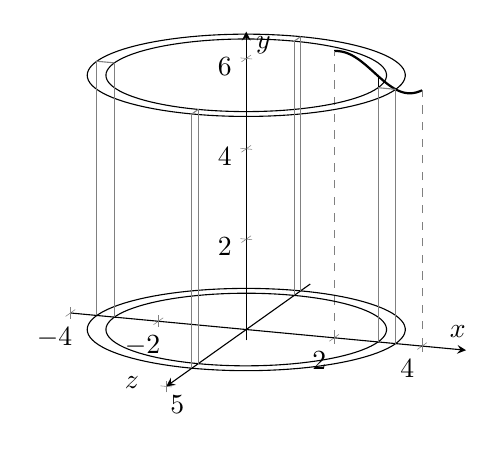
\begin{tikzpicture}
		\begin{axis}[
			view = {20}{15},
			axis equal,
			axis lines = center,
			xlabel = $x$,
			ylabel = $z$,
			y dir = reverse,
			zlabel = $y$,
			xmin = -4,
			xmax = 5,
			ymin = 0,
			ymax = 1,
  		every axis y label/.append style = {at = (ticklabel* cs:0)}]
			zmin = 0,
			zmax = 1.3,
			]
			\addplot3[
				samples = 50,
				domain = 2:4,
				domain y = 0:0,
				black,
				solid,
				thick
			](x, 0, {0.05*(x+5)*sin((2*(x+5))r)+6});
			\addplot3[
				gray,
				dashed
			]coordinates{(2, 0, 0) (2, 0, 6.34671)};
			\addplot3[
				gray,
				dashed
			]coordinates{(4, 0, 0) (4, 0, 5.66206)};
			\addplot3[
				black,
				solid
			]coordinates{(3, 0, 0) (3, 0, 5.88484)};
			\addplot3[
				black,
				solid
			]coordinates{(3.4, 0, 0) (3.4, 0, 5.62722)};
			\addplot3[
			samples = 100,
			domain = 0:2*pi,
			y domain = 0:0,
			black,
			solid
			]({3*cos(deg(x))}, {3*sin(deg(x))}, {5.62722});
			\addplot3[
			samples = 100,
			domain = 0:2*pi,
			y domain = 0:0,
			black,
			solid
			]({3.4*cos(deg(x))}, {3.4*sin(deg(x))}, {5.62722});
			\addplot3[
			samples = 100,
			domain = 0:2*pi,
			y domain = 0:0,
			black,
			solid
			]({3*cos(deg(x))}, {3*sin(deg(x))}, {0});
			\addplot3[
			samples = 100,
			domain = 0:2*pi,
			y domain = 0:0,
			black,
			solid
			]({3.4*cos(deg(x))}, {3.4*sin(deg(x))}, {0});
			\foreach \xx in {1.5708, 3.14159, ..., 6.2832}
			{
				\addplot3[
					gray,
					solid
				]coordinates{({3*cos(deg(\xx))}, {3*sin(deg(\xx))}, 0) ({3*cos(deg(\xx))}, {3*sin(deg(\xx))}, {5.62722})};
				\addplot3[
					gray,
					solid
				]coordinates{({3.4*cos(deg(\xx))}, {3.4*sin(deg(\xx))}, 0) ({3.4*cos(deg(\xx))}, {3.4*sin(deg(\xx))}, {5.62722})};
				\addplot3[
					gray,
					solid
				]coordinates{({3*cos(deg(\xx))}, {3*sin(deg(\xx))}, {5.62722}) ({3.4*cos(deg(\xx))}, {3.4*sin(deg(\xx))}, {5.62722})};
			}
		\end{axis}
	\end{tikzpicture}
	\caption{Creating the cylindrical shells.}
	\label{lec13:cylindermethod}
\end{figure}

What we do instead is to imagine making a cylindrical shell around the $y$-axis, constructed in such a way that the outer radius is $x_i$, the width of the shell is $\Delta x_i$, and the height is $f(x_i)$, as in Figure \ref{lec13:cylindermethod}.

Therefore the area of the rectangle we sweep around the $y$-axis is $f(x_i) \Delta x_i$.
When rotating this around the $y$-axis, we multiply by $2 \pi x_i$, since $x$ is the radius, and so the volume of the shell is
\[
	V(x_i) = 2 \pi x_i f(x_i) \Delta x_i.
\]
If we sum these for infinitely many $x_i$ between $a$ and $b$ such that $\Delta x_i \to 0$, the volume is
\[
	V = 2 \pi \int_a^b x f(x) \, d x.
\]

\begin{example}
	Find the volume of the torus generated by rotating the disc of radius $r$ centred on the the point $(R, 0)$, such that $0 < r < R$ around the $y$-axis.

	The circle with centre $(R, 0)$ and radius $r$ has the equation $(x - R)^2 + y^2 = r^2$, so its upper semicircle is the graph of
	\[
		f(x) = \sqrt{r^2 - (x - R)^2},
	\]
	for $R - r \leq x \leq R + r$.

	Rotating this around the $y$-axis we get half of the torus, so we double the volume as well:
	\[
		V = 2 \cdot 2 \pi \int_{R - r}^{R + r} x \sqrt{r^2 - (x - R)^2} \, d x,
	\]
	which we solve using substitution using $u = x - R$, whereby $d u = d x$, and when $x = R \pm r$ we have $u = \pm r$, so
	\begin{align*}
		V &= 4 \pi \int_{-r}^r (u + R) \sqrt{r^2 - u^2} \, d u \\
		  &= 4 \pi \int_{-r}^r u \sqrt{r^2 - u^2} \, d x + 4 \pi R \int_{-r}^r \sqrt{r^2 - u^2} \, d x,
	\end{align*}
	wherein the first integrand is odd and we're integrating over a symmetric interval, so it is $0$.
	The second integral we deal with by noticing that it is simply the area of a semicircle of radius $r$, i.e. $\pi r^2 / 2$.
	Thus
	\[
		V = 4 \pi R \frac{\pi r^2}{2} = 2 \pi^2 r^2 R = (\pi r^2) (2 \pi R). \qedhere
	\]
\end{example}

\noindent
We can compute the volume of some quite exotic solids by considering first something describing the outside of it, then taking away something describing the inside.

\begin{example}
	Find the volume of the solid generated by rotating the region bounded by $y = \sqrt{x}$ and $y = x$ around the $x$-axis.

	We first find the limits of integration:
	\[
		x = \sqrt{x} \quad\Rightarrow\quad x^2 = x \quad\Leftrightarrow\quad x(x - 1) = 0,
	\]
	so $x = 0$ and $x = 1$, neither of which are negative, so both solve the original equation.
	Therefore
	\begin{align*}
		V &= \pi \int_0^1 \sqrt{x}^2 \, d x - \pi \int_0^1 x^2 \, d x = \pi \int_0^1 x \, d x - \pi \int_0^1 x^2 \, d x \\
		  &= \pi \Big ( \frac{x^2}{2} \Big ) \biggr \rvert_0^1 - \pi \Big ( \frac{x^3}{3} \Big ) \biggr \rvert_0^1 = \frac{\pi}{2} - \frac{\pi}{3} = \frac{\pi}{6}. \qedhere
	\end{align*}
\end{example}

\noindent
One should avoid falling into the trap of describing the volume using
\[
	V = \pi \int_0^1 (\sqrt{x} - x)^2 \, d x,
\]
becuause whilst $\sqrt{x} - x$ describes the height difference between the two curves, it does \emph{not} describe the radius of the discs we want to generate.
(If we try, we end up with $\pi / 30$ instead.)

Indeed, if we think about it, we find that this second integral instead gives us the volume of $\sqrt{x}$ as rotated around $y = x$.

\begin{example}
	Find the volume of the bowl, the outside contour of which is given by $y = \sin(x)$, for $0 \leq x \leq \pi/2$.

	We get
	\[
		V = 2 \pi \int_0^{\pi/2} x \sin(x) \, d x,
	\]
	which we integrate by parts by taking $U(x) = x$ and $V'(x) = \sin(x)$, so that $U'(x) = 1$ and $V(x) = - \cos(x)$.
	Then we have
	\begin{align*}
		V &= 2 \pi (- x \cos(x)) \Big \rvert_0^{\pi/2} + 2 \pi \int_0^{\pi/2} 1 \cdot \cos(x) \, d x \\
		  &= 0 + 2 \pi \sin(x) \Big \rvert_0^{\pi/2} = 2 \pi (1 - 0) = 2 \pi. \qedhere
	\end{align*}
\end{example}
